\subsection{Caso d'uso UC2: Autenticazione}
\begin{figure}[h] 
	\centering 
	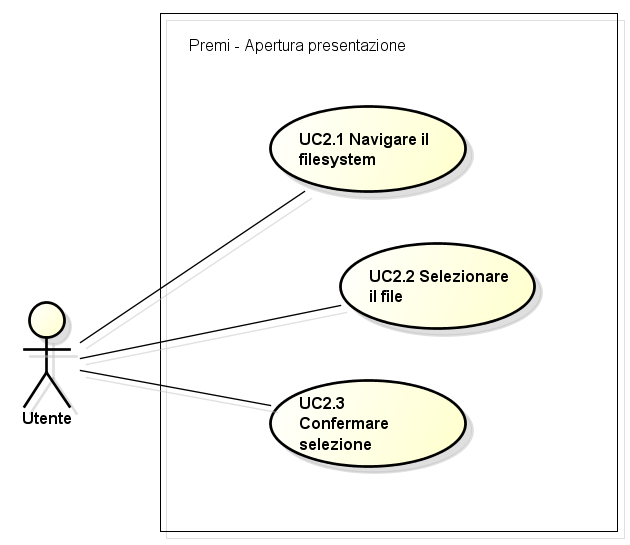
\includegraphics[scale=0.45] {img/UC2.png}
	\caption{UC2 - Autenticazione} 
\end{figure}

\begin{itemize}
	\item \textbf{Attori:} Utente non autenticato;
	\item \textbf{Scopo e descrizione:} L'utente è già iscritto e vuole avviare la procedura di autenticazione al sito per accedere ai propri file;
	\item \textbf{Precondizione:} L'utente ha selezionato la voce "accedi" presente sul sito;
	\item \textbf{Flusso principale degli eventi:}
	\begin{enumerate}
		\item L'utente inserisce le proprie credenziali [UC2.1];
		\item L'utente conferma l'inserimento dei dati selezionando la voce "login" [UC2.2];
		\item L'utente può recuperare le sue credenziali se le ha dimenticate [UC2.3].
	\end{enumerate}
	\item \textbf{Postcondizione:} Il sistema verifica le credenziali inserite e permette all'utente di accedere alla sua pagina personale.
\end{itemize}

\subsection{Caso d'uso UC2.1: Inserimento credenziali}
\begin{figure}[h] 
	\centering 
	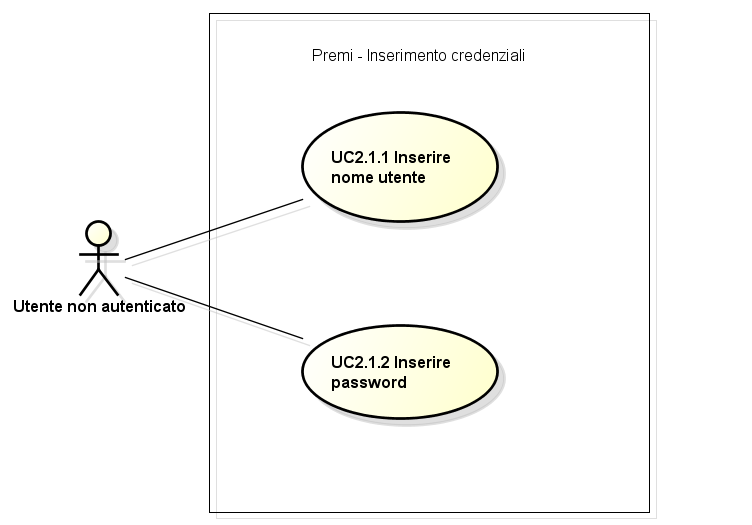
\includegraphics[scale=0.45] {img/UC2.1.png}
	\caption{UC2.1 - Inserimento credenziali} 
\end{figure}
\begin{itemize}
	\item \textbf{Attori:} Utente non autenticato;
	\item \textbf{Scopo e descrizione:} L'utente inserisce nome utente e password per poter accedere al sito;
	\item \textbf{Precondizione:} L'utente visualizza la schermata di inserimento dei dati richiesti per l'accesso;
	\item \textbf{Flusso principale degli eventi:}
	\begin{enumerate}
		\item L'utente inserisce il proprio nome utente [UC2.1.1];
		\item L'utente inserisce la propria password [UC2.1.2];
	\end{enumerate}
	\item \textbf{Postcondizione:} Tutti i campi richiesti sono stati compilati correttamente.
\end{itemize}

\subsection{Caso d'uso UC2.1.1: Inserire nome utente}
\begin{itemize}
	\item \textbf{Attori:} Utente non autenticato;
	\item \textbf{Scopo e descrizione:} L'utente inserisce il proprio nome utente;
	\item \textbf{Precondizione:} La casella dove inserire il nome utente è vuota;
	\item \textbf{Postcondizione:} La casella è stata compilata con il nome utente inserito dall'utente.
\end{itemize}

\subsection{Caso d'uso UC2.1.2: Inserire password}
\begin{itemize}
	\item \textbf{Attori:} Utente non autenticato;
	\item \textbf{Scopo e descrizione:} L'utente inserisce la propria password;
	\item \textbf{Precondizione:} La casella dove inserire la password è vuota;
	\item \textbf{Postcondizione:} La casella è stata compilata con la password inserita dall'utente.
\end{itemize}

\subsection{Caso d'uso UC2.2: Accesso}
\begin{itemize}
	\item \textbf{Attori:} Utente non autenticato;
	\item \textbf{Scopo e descrizione:} L'utente conferma le credenziali inserite scegliendo di effettuare l'accesso tramite il tasto di login;
	\item \textbf{Precondizione:} Nome utente e password sono stati inseriti;
	\item \textbf{Postcondizione:} Il sistema verifica i dati inseriti. Se sono corretti reindirizza l'utente alla pagina personale, altrimenti lo riporta alla schermata di accesso.
\end{itemize}

\subsection{Caso d'uso UC2.3: Recupero dati}
\begin{figure}[h] 
	\centering 
	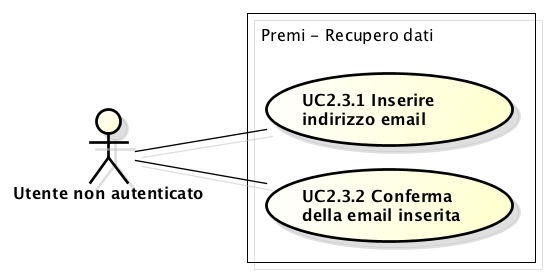
\includegraphics[scale=0.45] {img/UC2.3.png}
	\caption{UC2.3 - Recupero dati} 
\end{figure}
\begin{itemize}
	\item \textbf{Attori:} Utente non autenticato;
	\item \textbf{Scopo e descrizione:} L'utente non ricorda più le sue credenziali di accesso e sceglie quindi l'opzione per il recupero di tali dati. Il sistema gestirà la richiesta inviando all'indirizzo e-mail dell'utente tutti i suoi dati;
	\item \textbf{Precondizione:} L'utente ha selezionato l'opzione di recupero dei dati;
	\item \textbf{Flusso principale degli eventi:}
	\begin{enumerate}
		\item L'utente inserisce il proprio indirizzo mail [UC2.3.1];
		\item L'utente conferma l'inserimento dell'indirizzo mail [UC2.3.2];
		\item Il sistema controlla l'indirizzo e-mail inserita [UC2.3.3];
		\item Il sistema non trova l'indirizzo e-mail e segnala un errore [2.3.4];
		\item Il sistema trova una corrispondenza con l'indirizzo e-mail indicato e invia i dati [2.3.5].
	\end{enumerate}
	\item \textbf{Postcondizione:} Il sistema ha inviato una mail contenente i dati di accesso relativi all'utente che ne ha fatto richiesta.
\end{itemize}

\subsection{Caso d'uso UC2.3.1: Inserire indirizzo mail}
\begin{itemize}
	\item \textbf{Attori:} Utente non autenticato;
	\item \textbf{Scopo e descrizione:} L'utente inserisce il proprio indirizzo e-mail nella casella vuota;
	\item \textbf{Precondizione:} La casella dove inserire l'indirizzo e-mail è vuota;
	\item \textbf{Postcondizione:} La casella è stata compilata con l'indirizzo e-mail inserito dall'utente.
\end{itemize}

\subsection{Caso d'uso UC2.3.2: Conferma della mail inserita}
\begin{itemize}
	\item \textbf{Attori:} Utente non autenticato;
	\item \textbf{Scopo e descrizione:} L'utente conferma la mail inserita in precedenza e invia la richiesta;
	\item \textbf{Precondizione:} L'utente ha inserito un indirizzo e-mail;
	\item \textbf{Postcondizione:} L'utente ha confermato l'indirizzo e-mail inserito.
\end{itemize}
